\documentclass[11pt,openany]{article}

\input{crypto-preamble}
\usepackage{tcolorbox}
\tcbset{colback=white, arc=5pt}

\definecolor{axiomcolor}{HTML}{a88bfa}
\definecolor{defcolor}{RGB}{52, 152, 219}
\definecolor{procolor}{RGB}{241, 196, 15}
\definecolor{thmcolor}{RGB}{231, 76, 60}
\definecolor{lemcolor}{RGB}{155, 89, 182}
\definecolor{corcolor}{RGB}{46, 204, 113}
\definecolor{execolor}{RGB}{90, 128, 127}

% Define a new command for the custom tcolorbox
\newcommand{\axiombox}[2][]{%
	\begin{tcolorbox}[colframe=axiomcolor, title={\color{white}\bfseries #1}]
		#2
	\end{tcolorbox}
}

\newcommand{\defbox}[2][]{%
	\begin{tcolorbox}[colframe=defcolor, title={\color{white}\bfseries #1}]
		#2
	\end{tcolorbox}
}

\newcommand{\probox}[2][]{%
	\begin{tcolorbox}[colframe=procolor, title={\color{white}\bfseries #1}]
		#2
	\end{tcolorbox}
}

\newcommand{\thmbox}[2][]{%
	\begin{tcolorbox}[colframe=thmcolor, title={\color{white}\bfseries #1}]
		#2
	\end{tcolorbox}
}

\newcommand{\lembox}[2][]{%
	\begin{tcolorbox}[colframe=lemcolor, title={\color{white}\bfseries #1}]
		#2
	\end{tcolorbox}
}
\usepackage{amsthm}

% Define custom theorem styles
\newtheoremstyle{dotless} % Name of the style
{3pt} % Space above
{3pt} % Space below
{\itshape} % Body font
{} % Indent amount
{\bfseries} % Theorem head font
{} % Punctuation after theorem head
{2.5mm} % Space after theorem head
{} % Theorem head spec

\newtheoremstyle{definitionstyle} % Name of the style
{3pt} % Space above
{3pt} % Space below
{} % Body font
{} % Indent amount
{\bfseries} % Theorem head font
{.} % Punctuation after theorem head
{2.5mm} % Space after theorem head
{} % Theorem head spec

% Applying custom styles
%\theoremstyle{dotless}
\newtheorem{theorem}{Theorem} % Theorem environment with section-wise numbering
\newtheorem*{theorem*}{Theorem} % Theorem environment with section-wise numbering
\newtheorem*{lemma*}{Lemma} % Theorem environment with section-wise numbering
\newtheorem*{proposition*}{Proposition} % Theorem environment with section-wise numbering
\newtheorem*{corollary*}{Corollary} % Theorem environment with section-wise numbering
\newtheorem{proposition}[theorem]{Proposition} % Theorem environment with section-wise numbering
\newtheorem{lemma}[theorem]{Lemma} % Lemma shares the counter with theorem
\newtheorem{corollary}[theorem]{Corollary} % Corollary shares the counter with theorem

\theoremstyle{definitionstyle}
\newtheorem*{observation}{\textcolor{magenta}{Observation}}
\newtheorem*{illustration}{\textcolor{teal}{Illustration}}
\newtheorem*{torus}{{\color{red}T}{\color{orange}o}{\color{green!75!black}r}{\color{cyan}u}{\color{violet}s}}
\newtheorem{definition}{Definition} % Definition shares the counter with theorem
\newtheorem{example}{Example} % Example shares the counter with theorem
\newtheorem{exercise}{{Exercise}} % Example shares the counter with theorem
\newtheorem{remark}{Remark} % Remark shares the counter with theorem
\newtheorem*{note}{Note}
\newtheorem*{notation}{Notation}

\newtheorem*{axiom*}{Axiom}
\newtheorem*{definition*}{Definition} % Definition shares the counter with theorem
\newtheorem*{example*}{Example} % Example shares the counter with theorem
\newtheorem*{exercise*}{\textcolor{teal}{Exercise}} % Example shares the counter with theorem
\newtheorem*{remark*}{Remark} % Remark shares the counter with theorem


\usepackage{tikz}
\usepackage{tikz-cd}
\usetikzlibrary{shadows}
\usetikzlibrary{shapes.geometric, arrows.meta, positioning}
\input{crypto-commands}
\renewcommand{\vec}[1]{\mathbf{#1}}
\renewcommand{\Re}{\operatorname*{Re}}
\renewcommand{\Im}{\operatorname*{Im}}
\newcommand{\rank}{\mathrm{rank}}
%\newcommand{\Mat}{\operatorname{Mat}}

\newcommand{\Sym}{\mathrm{Sym}}

\setstretch{1.25}

\begin{document}
\pagenumbering{arabic}
\begin{center}
	\huge\textbf{Rijndael S-Box}\\
	\vspace{0.5em}
	\large{Ji, Yong-hyeon}\\
	\vspace{0.5em}
	\normalsize{\today}\\
\end{center}

\noindent 
We cover the following topics in this note.
\begin{itemize}
	\item Rijndael S-Box
	\item Vector Space $\F_2=\set{0,1}$
\end{itemize}
\hrule\vspace{12pt}
%\tableofcontents
\vfill
\begin{table}[h]
\centering\ttfamily\renewcommand{\arraystretch}{1.5}
\begin{tabular}{c|*{16}{c}}
	\toprule[1.2pt]
	& 0 & 1 & 2 & 3 & 4 & 5 & 6 & 7 & 8 & 9 & a & b & c & d & e & f \\
	\hline
	0 & 63 & 7c & 77 & 7b & f2 & 6b & 6f & c5 & 30 & 01 & 67 & 2b & fe & d7 & ab & 76 \\
	1 & ca & 82 & c9 & 7d & fa & 59 & 47 & f0 & ad & d4 & a2 & af & 9c & a4 & 72 & c0 \\
	2 & b7 & fd & 93 & 26 & 36 & 3f & f7 & cc & 34 & a5 & e5 & f1 & 71 & d8 & 31 & 15 \\
	3 & 04 & c7 & 23 & c3 & 18 & 96 & 05 & 9a & 07 & 12 & 80 & e2 & eb & 27 & b2 & 75 \\
	4 & 09 & 83 & 2c & 1a & 1b & 6e & 5a & a0 & 52 & 3b & d6 & b3 & 29 & e3 & 2f & 84 \\
	5 & 53 & d1 & 00 & ed & 20 & fc & b1 & 5b & 6a & cb & be & 39 & 4a & 4c & 58 & cf \\
	6 & d0 & ef & aa & fb & 43 & 4d & 33 & 85 & 45 & f9 & 02 & 7f & 50 & 3c & 9f & a8 \\
	7 & 51 & a3 & 40 & 8f & 92 & 9d & 38 & f5 & bc & b6 & da & 21 & 10 & ff & f3 & d2 \\
	8 & cd & 0c & 13 & ec & 5f & 97 & 44 & 17 & c4 & a7 & 7e & 3d & 64 & 5d & 19 & 73 \\
	9 & 60 & 81 & 4f & dc & 22 & 2a & 90 & 88 & 46 & ee & b8 & 14 & de & 5e & 0b & db \\
	a & e0 & 32 & 3a & 0a & 49 & 06 & 24 & 5c & c2 & d3 & ac & 62 & 91 & 95 & e4 & 79 \\
	b & e7 & c8 & 37 & 6d & 8d & d5 & 4e & a9 & 6c & 56 & f4 & ea & 65 & 7a & ae & 08 \\
	c & ba & 78 & 25 & 2e & 1c & a6 & b4 & c6 & e8 & dd & 74 & 1f & 4b & bd & 8b & 8a \\
	d & 70 & 3e & b5 & 66 & 48 & 03 & f6 & 0e & 61 & 35 & 57 & b9 & 86 & c1 & 1d & 9e \\
	e & e1 & f8 & 98 & 11 & 69 & d9 & 8e & 94 & 9b & 1e & 87 & e9 & ce & 55 & 28 & df \\
	f & 8c & a1 & 89 & 0d & bf & e6 & 42 & 68 & 41 & 99 & 2d & 0f & b0 & 54 & bb & 16 \\
	\bottomrule[1.2pt]
\end{tabular}
\caption{\normalfont AES S-box values in hexadecimal}
\end{table}

\newpage
\begin{table}[h]
\centering\ttfamily\renewcommand{\arraystretch}{1.5}
\begin{tabular}{c|*{16}{c}}
	\toprule[1.2pt]
	& 0 & 1 & 2 & 3 & 4 & 5 & 6 & 7 & 8 & 9 & a & b & c & \cellcolor{-red}d & e & f \\
	\hline
	0 & 63 & 7c & 77 & 7b & f2 & 6b & 6f & c5 & 30 & 01 & 67 & 2b & fe & d7 & ab & 76 \\
	1 & ca & 82 & c9 & 7d & fa & 59 & 47 & f0 & ad & d4 & a2 & af & 9c & a4 & 72 & c0 \\
	2 & b7 & fd & 93 & 26 & 36 & 3f & f7 & cc & 34 & a5 & e5 & f1 & 71 & d8 & 31 & 15 \\
	3 & 04 & c7 & 23 & c3 & 18 & 96 & 05 & 9a & 07 & 12 & 80 & e2 & eb & 27 & b2 & 75 \\
	4 & 09 & 83 & 2c & 1a & 1b & 6e & 5a & a0 & 52 & 3b & d6 & b3 & 29 & e3 & 2f & 84 \\
	5 & 53 & d1 & 00 & ed & 20 & fc & b1 & 5b & 6a & cb & be & 39 & 4a & 4c & 58 & cf \\
	6 & d0 & ef & aa & fb & 43 & 4d & 33 & 85 & 45 & f9 & 02 & 7f & 50 & 3c & 9f & a8 \\
	\cellcolor{-red}7 & 51 & a3 & 40 & 8f & 92 & 9d & 38 & f5 & bc & b6 & da & 21 & 10 & \cellcolor{-red}ff & f3 & d2 \\
	8 & cd & 0c & 13 & ec & 5f & 97 & 44 & 17 & c4 & a7 & 7e & 3d & 64 & 5d & 19 & 73 \\
	9 & 60 & 81 & 4f & dc & 22 & 2a & 90 & 88 & 46 & ee & b8 & 14 & de & 5e & 0b & db \\
	a & e0 & 32 & 3a & 0a & 49 & 06 & 24 & 5c & c2 & d3 & ac & 62 & 91 & 95 & e4 & 79 \\
	b & e7 & c8 & 37 & 6d & 8d & d5 & 4e & a9 & 6c & 56 & f4 & ea & 65 & 7a & ae & 08 \\
	c & ba & 78 & 25 & 2e & 1c & a6 & b4 & c6 & e8 & dd & 74 & 1f & 4b & bd & 8b & 8a \\
	d & 70 & 3e & b5 & 66 & 48 & 03 & f6 & 0e & 61 & 35 & 57 & b9 & 86 & c1 & 1d & 9e \\
	e & e1 & f8 & 98 & 11 & 69 & d9 & 8e & 94 & 9b & 1e & 87 & e9 & ce & 55 & 28 & df \\
	f & 8c & a1 & 89 & 0d & bf & e6 & 42 & 68 & 41 & 99 & 2d & 0f & b0 & 54 & bb & 16 \\
	\bottomrule[1.2pt]
\end{tabular}
%\caption{\normalfont AES S-box values in hexadecimal}
\end{table}
\begin{center}
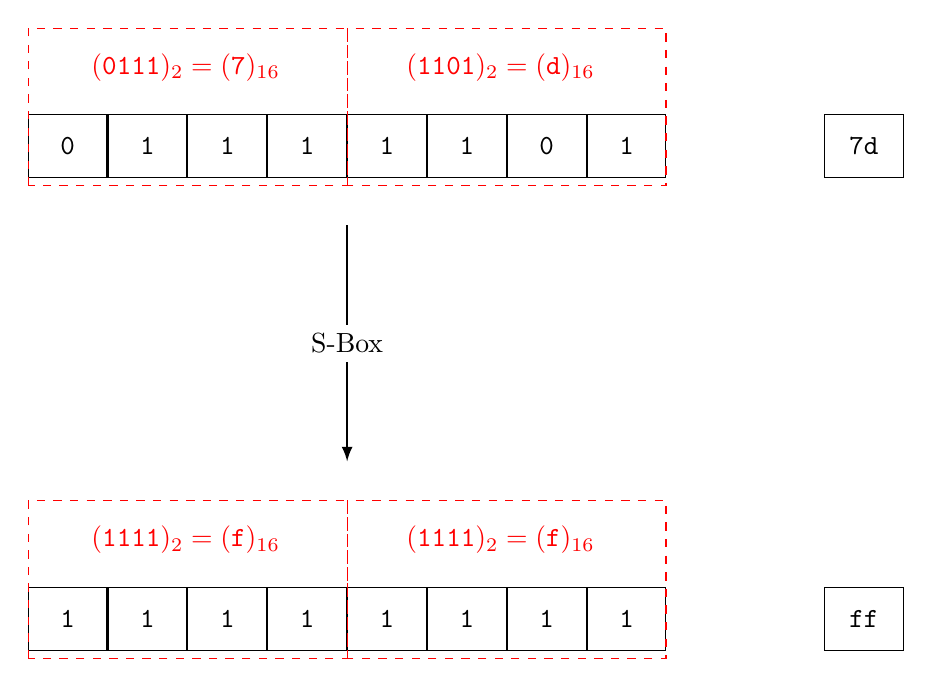
\begin{tikzpicture}[
	box/.style={draw, minimum width=1cm, minimum height=0.8cm, align=center},
	>=latex
	]
	\node[box] (a0) at (0,2) {$\texttt{0}$};
	\node[box] (a1) [right=0 of a0] {$\texttt{1}$};
	\node[box] (a2) [right=0 of a1] {$\texttt{1}$};
	\node[box] (a3) [right=0 of a2] {$\texttt{1}$};
	\node[box] (a4) [right=0 of a3] {$\texttt{1}$};
	\node[box] (a5) [right=0 of a4] {$\texttt{1}$};
	\node[box] (a6) [right=0 of a5] {$\texttt{0}$};
	\node[box] (a7) [right=0 of a6] {$\texttt{1}$};
	\node[box] (a8) [right=2 of a7] {$\texttt{7d}$};
	\node[red] at (1.5,3)
	{$(\texttt{0111})_2=(\texttt{7})_{16}$};
	\node[red] at (5.5,3)
	{$(\texttt{1101})_2=(\texttt{d})_{16}$};
	\draw[red, dashed] (-.5,1.5) rectangle (3.55,3.5);
	\draw[red, dashed] (3.55,1.5) rectangle (7.6,3.5);
	
	\draw[->, thick] (3.55,1) -- ++(0,-3) node[midway, fill=white] {S-Box};
	
	\begin{scope}[yshift=-6cm]
	\node[box] (a0) at (0,2) {$\texttt{1}$};
	\node[box] (a1) [right=0 of a0] {$\texttt{1}$};
	\node[box] (a2) [right=0 of a1] {$\texttt{1}$};
	\node[box] (a3) [right=0 of a2] {$\texttt{1}$};
	\node[box] (a4) [right=0 of a3] {$\texttt{1}$};
	\node[box] (a5) [right=0 of a4] {$\texttt{1}$};
	\node[box] (a6) [right=0 of a5] {$\texttt{1}$};
	\node[box] (a7) [right=0 of a6] {$\texttt{1}$};
	\node[box] (a8) [right=2 of a7] {$\texttt{ff}$};
	\node[red] at (1.5,3)
	{$(\texttt{1111})_2=(\texttt{f})_{16}$};
	\node[red] at (5.5,3)
	{$(\texttt{1111})_2=(\texttt{f})_{16}$};
	\draw[red, dashed] (-.5,1.5) rectangle (3.55,3.5);
	\draw[red, dashed] (3.55,1.5) rectangle (7.6,3.5);
	\end{scope}
\end{tikzpicture}
\end{center}

\newpage\noindent
We work in the finite field \(\mathbb{F}_{2^8}\), represented as
\(\mathbb{F}_2^8\) via some fixed \(\mathbb{F}_2\)-linear isomorphism.
The AES S-box (up to the special convention at \(0\)) can be written as
\[
S(x) = A(x^{-1}) + b,
\]
where
\begin{itemize}
	\item \(x^{-1}\) is the multiplicative inverse in \(\mathbb{F}_{2^8}\),
	with the convention \(0^{-1} := 0\),
	\begin{itemize}
		\item $\mathbb{F}_{2^8} \cong \mathbb{F}_2[x]/\bigl(x^8 + x^4 + x^3 + x + 1\bigr)$
	\end{itemize}
	\item \(A : \mathbb{F}_2^8 \to \mathbb{F}_2^8\) is an invertible
	\(\mathbb{F}_2\)-linear map (given by an \(8\times 8\) matrix
	over \(\mathbb{F}_2\)),
	\item \(b \in \mathbb{F}_2^8\) is a fixed constant (an ``offset'').
\end{itemize}

%\newpage
%We now describe the role of each component.
%
%\subsubsection*{(1) The map \(x \mapsto x^{-1}\): source of nonlinearity}
%
%On the multiplicative group \(\mathbb{F}_{2^8}^\times\), the map
%\[
%f(x) = x^{-1}
%\]
%is a permutation with inverse \(f^{-1}=f\).
%Viewed (via coordinates) as a function
%\(\tilde{f} : \mathbb{F}_2^8 \to \mathbb{F}_2^8\),
%this is a highly nonlinear permutation with the following properties:
%
%\begin{itemize}
%	\item It is \emph{not} \(\mathbb{F}_2\)-linear or affine:
%	no nontrivial linear relation of the form
%	\(L(x^{-1}) = L'(x)\) holds with linear \(L,L'\).
%	\item It has low differential uniformity:
%	for each nonzero \(a \in \mathbb{F}_{2^8}\), the number of
%	solutions \(x\) to \(x^{-1} + (x+a)^{-1} = b\) is uniformly small.
%	\item It has high nonlinearity as a vectorial Boolean function:
%	each coordinate bit of \(\tilde{f}\) is far (in Hamming distance)
%	from every affine function of the input bits.
%\end{itemize}
%
%Thus, \(x \mapsto x^{-1}\) is the \emph{essential nonlinear core}
%of the S-box, responsible for resisting linear and differential attacks.
%
%\subsubsection*{(2) The linear map \(A\): mixing and shaping the output}
%
%The map
%\[
%L(z) := A z,\qquad A \in \mathrm{GL}(8,2),
%\]
%is \(\mathbb{F}_2\)-linear and invertible. Applied after inversion,
%it yields the composition
%\[
%x \longmapsto L(x^{-1}) = A(x^{-1}).
%\]
%
%The role of \(A\) is:
%
%\begin{itemize}
%	\item \textbf{Bit mixing / diffusion.}
%	Over \(\mathbb{F}_2^8\), each output bit of \(A(x^{-1})\) is a
%	linear combination of many bits of \(x^{-1}\).
%	This spreads the influence of each input bit across several output bits,
%	improving diffusion.
%	
%	\item \textbf{Shaping linear properties without weakening nonlinearity.}
%	Since \(A\) is linear and invertible, composing with \(A\) does \emph{not}
%	change fundamental measures such as differential uniformity or nonlinearity:
%	these are invariant under composition with affine bijections.
%	However, \(A\) can be chosen to optimize linear-algebraic criteria
%	such as branch number or the distribution of Hamming weights.
%	
%	\item \textbf{Change of coordinates.}
%	Conceptually, \(A\) corresponds to a change of basis in the underlying
%	\(\mathbb{F}_2\)-vector space. Different choices of \(A\) yield
%	affine-equivalent S-boxes with the same cryptographic strength but
%	different bit-level structure and implementation cost.
%\end{itemize}
%
%Thus, \(A\) uses only \emph{linear} operations to improve the way the
%nonlinearity of inversion is ``seen'' at the bit level, while preserving
%invertibility and the good nonlinear properties of the core.
%
%\subsubsection*{(3) Addition of the constant \(b\): translation and symmetry breaking}
%
%Finally, one adds a constant vector \(b \in \mathbb{F}_2^8\) and defines
%\[
%S(x) = A(x^{-1}) + b.
%\]
%
%Because addition of a fixed vector is an affine translation, this step has
%the following effects:
%
%\begin{itemize}
%	\item \textbf{Preservation of difference propagation.}
%	For all \(x,y \in \mathbb{F}_2^8\),
%	\[
%	S(x) + S(y)
%	= \bigl(A(x^{-1}) + b\bigr) + \bigl(A(y^{-1}) + b\bigr)
%	= A(x^{-1} + y^{-1}),
%	\]
%	so the constant \(b\) cancels in differences.
%	Hence, differential properties are unchanged by the addition of \(b\).
%	
%	\item \textbf{No fixed points or simple linear relations.}
%	By choosing \(b\) suitably, one can ensure that \(S\) has no fixed
%	points of the form \(S(x)=x\), or other undesirable patterns such as
%	\(S(0)=0\) or \(S(x) = x^{-1}\) for many \(x\).
%	This helps avoid simple algebraic or structural weaknesses.
%	
%	\item \textbf{Cosmetic randomization.}
%	The choice of \(b\) makes the output values appear more ``random''
%	from a tabular (lookup) point of view, without altering the underlying
%	combinatorial strength induced by the inversion and the linear map \(A\).
%\end{itemize}
%
%In summary:
%\begin{itemize}
%	\item \(x \mapsto x^{-1}\) provides the core nonlinearity in \(\mathbb{F}_{2^8}\),
%	\item multiplication by \(A\) linearly mixes and reshapes this nonlinearity
%	at the bit level, while preserving cryptographic measures such as
%	nonlinearity and differential uniformity,
%	\item addition of \(b\) translates the output to remove simple symmetries
%	and fixed points, again without affecting differential behaviour.
%\end{itemize}
%
%\newpage
%\subsection{Why Use the Multiplicative Inverse in \texorpdfstring{$\mathbb{F}_{2^8}$}{GF(2^8)}?}
%
%The AES S-box is built from the multiplicative inverse in the finite field
%\[
%\mathbb{F}_{2^8} \cong \mathbb{F}_2[x]/\bigl(x^8 + x^4 + x^3 + x + 1\bigr).
%\]
%We briefly justify this choice from a finite-field and cryptographic point of view.
%
%\subsubsection{Field Representation and Coordinates}
%
%Let \(p(x) = x^8 + x^4 + x^3 + x + 1 \in \mathbb{F}_2[x]\). The polynomial \(p(x)\) is irreducible
%over \(\mathbb{F}_2\), hence the quotient ring
%\[
%\mathbb{F}_{2^8} := \mathbb{F}_2[x]/(p(x))
%\]
%is a field of \(2^8 = 256\) elements.
%
%Every element of \(\mathbb{F}_{2^8}\) can be written uniquely as
%\[
%a_0 + a_1 x + \cdots + a_7 x^7,\quad a_i \in \mathbb{F}_2,
%\]
%so that we have an \(\mathbb{F}_2\)-vector space isomorphism
%\[
%\varphi : \mathbb{F}_{2^8} \longrightarrow \mathbb{F}_2^8,\qquad
%a_0 + a_1 x + \cdots + a_7 x^7 \,\longmapsto\,
%(a_0,\dots,a_7)^{\mathsf T}.
%\]
%This is just a choice of coordinates (a basis) for the \(8\)-dimensional vector space.
%
%\subsubsection{The Inversion Map as a Nonlinear Permutation}
%
%On the multiplicative group \(\mathbb{F}_{2^8}^\times = \mathbb{F}_{2^8} \setminus \{0\}\), the map
%\[
%f : \mathbb{F}_{2^8}^\times \to \mathbb{F}_{2^8}^\times,\qquad
%f(a) = a^{-1},
%\]
%is a permutation with inverse \(f^{-1} = f\). Extending by a convention at \(0\), e.g.
%\[
%S(a) :=
%\begin{cases}
%	a^{-1}, & a \neq 0,\\
%	0, & a = 0,
%\end{cases}
%\]
%we obtain a permutation \(S : \mathbb{F}_{2^8} \to \mathbb{F}_{2^8}\).
%
%Via the coordinate isomorphism \(\varphi\), this induces a permutation of bytes:
%\[
%\tilde{S} := \varphi \circ S \circ \varphi^{-1} : \mathbb{F}_2^8 \to \mathbb{F}_2^8.
%\]
%This is the core nonlinear map in the S-box.
%
%\subsubsection{Cryptographic Properties of the Inversion Map}
%
%The function \(a \mapsto a^{-1}\) in \(\mathbb{F}_{2^m}\) has several properties that make it
%extremely suitable as the nonlinear part of an S-box:
%
%\begin{enumerate}
%	\item \textbf{Permutation.} It is a bijection on \(\mathbb{F}_{2^8}\), so it can be used directly
%	inside a block cipher without losing invertibility.
%	
%	\item \textbf{Good differential properties.}
%	For \(a \in \mathbb{F}_{2^8}\), \(a \neq 0\), and any \(b \in \mathbb{F}_{2^8}\), one studies
%	the number of solutions \(x \in \mathbb{F}_{2^8}\) of the \emph{differential equation}
%	\[
%	f(x+a) + f(x) = b,
%	\]
%	where addition is in \(\mathbb{F}_{2^8}\).
%	The inversion map has (provably) low differential uniformity; in particular, it is
%	``almost optimal'' among permutations for resisting differential cryptanalysis.
%	
%	\item \textbf{High nonlinearity.}
%	Viewing \(\tilde{S} : \mathbb{F}_2^8 \to \mathbb{F}_2^8\) as a vectorial Boolean function,
%	each output bit is a Boolean function of 8 variables. These Boolean functions have
%	\emph{high nonlinearity} (large distance from all affine functions), which provides
%	resistance to linear cryptanalysis.
%	
%	\item \textbf{High algebraic degree.}
%	Over \(\mathbb{F}_2\), the algebraic degree of the coordinate functions of the inversion map
%	is maximal (or near maximal) for dimension \(8\), which makes it harder to approximate
%	by low-degree polynomials and strengthens resistance to certain algebraic attacks.
%\end{enumerate}
%
%In short: among all permutations on \(256\) elements, the inversion in \(\mathbb{F}_{2^8}\) is
%distinguished by excellent differential and linear properties, algebraic degree, and the fact
%that it can be described and implemented in a mathematically concise way.
%
%\subsubsection{Why This Specific Polynomial \texorpdfstring{$x^8 + x^4 + x^3 + x + 1$}{x8 + x4 + x3 + x + 1}?}
%
%The choice of the irreducible polynomial
%\[
%p(x) = x^8 + x^4 + x^3 + x + 1
%\]
%does \emph{not} change the abstract finite field \(\mathbb{F}_{2^8}\) up to isomorphism: any two
%irreducible polynomials of degree \(8\) over \(\mathbb{F}_2\) yield isomorphic fields.
%
%From the cryptographic point of view, changing the field representation
%\[
%\mathbb{F}_{2^8} \cong \mathbb{F}_2^8
%\]
%by another basis (i.e.\ by another isomorphism \(\varphi\)) simply conjugates the inversion map
%by a linear isomorphism. This produces an \emph{affine-equivalent} S-box with the same
%differential and linear properties. Thus, the concrete choice of \(p(x)\) is largely an
%implementation/detail choice (e.g.\ for efficient hardware realization), not a change in the
%fundamental nonlinearity mechanism.
%
%\subsubsection{Summary}
%
%The S-box of AES uses inversion in the finite field \(\mathbb{F}_{2^8}\) because:
%
%\begin{itemize}
%	\item inversion is a bijective map with excellent differential and linear properties,
%	\item it yields a compact, algebraically defined source of strong nonlinearity,
%	\item the field \(\mathbb{F}_{2^8}\) is naturally suited to \(8\)-bit bytes,
%	\item the specific polynomial \(x^8 + x^4 + x^3 + x + 1\) is a convenient way to represent
%	\(\mathbb{F}_{2^8}\), chosen primarily for implementation efficiency.
%\end{itemize}
%
%An additional affine transformation is applied after inversion to remove fixed points and
%further improve certain structural properties, but the essential nonlinearity comes from the
%map \(a \mapsto a^{-1}\) in \(\mathbb{F}_{2^8}\).
%
%
%
%
%\newpage
%%\subsection*{Operations on \texorpdfstring{$\mathbb{F}_2$}{F\_2}}
%%
%%We recall that
%%\[
%%\mathbb{F}_2 := \{0,1\}
%%\]
%%with addition and multiplication defined modulo \(2\).
%%
%%\paragraph{Addition.}
%%For \(a,b \in \mathbb{F}_2\), the sum \(a + b\) is given by
%%\[
%%0 + 0 = 0,\quad
%%0 + 1 = 1,\quad
%%1 + 0 = 1,\quad
%%1 + 1 = 0.
%%\]
%%Equivalently,
%%\[
%%a + b \equiv a + b \pmod{2},
%%\]
%%so that \(1 + 1 = 0\) in \(\mathbb{F}_2\). In computer-science terms, this is the bitwise XOR operation on single bits.
%%
%%\paragraph{Multiplication.}
%%For \(a,b \in \mathbb{F}_2\), the product \(ab\) is given by
%%\[
%%0 \cdot 0 = 0,\quad
%%0 \cdot 1 = 0,\quad
%%1 \cdot 0 = 0,\quad
%%1 \cdot 1 = 1.
%%\]
%%Equivalently,
%%\[
%%ab \equiv ab \pmod{2},
%%\]
%%so the element \(1\) is the multiplicative identity and \(0\) is the absorbing element.
%%
%%With these operations, \(\mathbb{F}_2\) is a field: \((\mathbb{F}_2,+)\) is an abelian group, \((\mathbb{F}_2\setminus\{0\},\cdot)\) is an abelian group, and multiplication distributes over addition.
%%
%%\subsection{Operations on the Vector Space \texorpdfstring{$\mathbb{F}_2^8$}{F\_2^8}}
%%
%%We now consider the \(8\)-dimensional vector space
%%\[
%%\mathbb{F}_2^8 := \{(x_0,\dots,x_7)^{\mathsf{T}} : x_i \in \mathbb{F}_2\}.
%%\]
%%
%%\paragraph{Vector addition.}
%%Given two vectors
%%\[
%%x = \begin{bmatrix} x_0 \\ x_1 \\ \vdots \\ x_7 \end{bmatrix},
%%\quad
%%y = \begin{bmatrix} y_0 \\ y_1 \\ \vdots \\ y_7 \end{bmatrix}
%%\in \mathbb{F}_2^8,
%%\]
%%their sum \(x + y\) is defined componentwise using addition in \(\mathbb{F}_2\):
%%\[
%%x + y :=
%%\begin{bmatrix}
%%	x_0 + y_0 \\
%%	x_1 + y_1 \\
%%	\vdots \\
%%	x_7 + y_7
%%\end{bmatrix},
%%\]
%%where each \(x_i + y_i\) is computed modulo \(2\).
%%In particular, each coordinate sum is the XOR of the corresponding bits.
%%
%%\paragraph{Scalar multiplication.}
%%Scalars are elements of \(\mathbb{F}_2 = \{0,1\}\). For \(\lambda \in \mathbb{F}_2\) and \(x \in \mathbb{F}_2^8\),
%%\[
%%\lambda \cdot x :=
%%\begin{bmatrix}
%%	\lambda x_0 \\
%%	\lambda x_1 \\
%%	\vdots \\
%%	\lambda x_7
%%\end{bmatrix},
%%\]
%%where each product \(\lambda x_i\) is the product in \(\mathbb{F}_2\). Explicitly,
%%\[
%%0 \cdot x =
%%\begin{bmatrix} 0 \\ 0 \\ \vdots \\ 0 \end{bmatrix},
%%\qquad
%%1 \cdot x = x
%%\quad\text{for all } x \in \mathbb{F}_2^8.
%%\]
%%
%%With these two operations, \(\mathbb{F}_2^8\) is a vector space of dimension \(8\) over the field \(\mathbb{F}_2\).
%%
%%%\medskip
%%%
%%%\noindent
%%%\textbf{Remark.}
%%%In this notation, \(\mathbb{F}_2^8\) denotes the \(8\)-dimensional \emph{vector space} over \(\mathbb{F}_2\) with componentwise addition and scalar multiplication as above. By contrast, the notation \(\mathbb{F}_{2^8}\) usually denotes a field extension of degree \(8\) of \(\mathbb{F}_2\), equipped with an additional (non-componentwise) field multiplication. In the present linear-algebraic discussion we work with \(\mathbb{F}_2^8\) as a vector space.

\newpage
\begin{align*}
\text{S-Box:}&\qquad\begin{bmatrix}s_0\\s_1\\s_2\\s_3\\s_4\\s_5\\s_6\\s_7\end{bmatrix} =
\begin{bmatrix}
	1 & 0 & 0 & 0 & 1 & 1 & 1 & 1 \\
	1 & 1 & 0 & 0 & 0 & 1 & 1 & 1 \\
	1 & 1 & 1 & 0 & 0 & 0 & 1 & 1 \\
	1 & 1 & 1 & 1 & 0 & 0 & 0 & 1 \\
	1 & 1 & 1 & 1 & 1 & 0 & 0 & 0 \\
	0 & 1 & 1 & 1 & 1 & 1 & 0 & 0 \\
	0 & 0 & 1 & 1 & 1 & 1 & 1 & 0 \\
	0 & 0 & 0 & 1 & 1 & 1 & 1 & 1
\end{bmatrix}\begin{bmatrix}
	b_0\\ b_1\\ b_2\\ b_3\\ b_4\\ b_5\\ b_6\\ b_7
\end{bmatrix} + \begin{bmatrix}
	1 \\ 1\\ 0\\ 0\\ 0\\ 1\\ 1\\ 0
\end{bmatrix}
%\\ \\
%\text{Inverse S-Box:}&\qquad\begin{bmatrix} b_0\\ b_1\\ b_2\\ b_3\\ b_4\\ b_5\\ b_6\\ b_7\end{bmatrix} =
%\begin{bmatrix}
%	0 & 0 & 1 & 0 & 0 & 1 & 0 & 1 \\
%	1 & 0 & 0 & 1 & 0 & 0 & 1 & 0 \\
%	0 & 1 & 0 & 0 & 1 & 0 & 0 & 1 \\
%	1 & 0 & 1 & 0 & 0 & 1 & 0 & 0 \\
%	0 & 1 & 0 & 1 & 0 & 0 & 1 & 0 \\
%	0 & 0 & 1 & 0 & 1 & 0 & 0 & 1 \\
%	1 & 0 & 0 & 1 & 0 & 1 & 0 & 0 \\
%	0 & 1 & 0 & 0 & 1 & 0 & 1 & 0
%\end{bmatrix}
%\begin{bmatrix}
%	s_0\\ s_1\\ s_2\\ s_3\\ s_4\\ s_5\\ s_6\\ s_7
%\end{bmatrix} + \begin{bmatrix}
%	1\\ 0\\ 1\\ 0\\ 0\\ 0\\ 0\\ 0
%\end{bmatrix}
\end{align*}
This transformation is the sum of multiple rotations of the byte as a vector, where addition is the XOR operation: \[
s = b \oplus (b \lll 1) \oplus (b \lll 2) \oplus (b \lll 3) \oplus (b \lll 4) \oplus \texttt{63}_{16}
\]
where $b$ represents the multiplicative inverse, $\oplus$ is the bitwise XOR operator, $\lll$ is a left bitwise circular shift, and the constant $\texttt{63}_{16}=\texttt{01100011}_2$ is given in hexadecimal.
\begin{center}
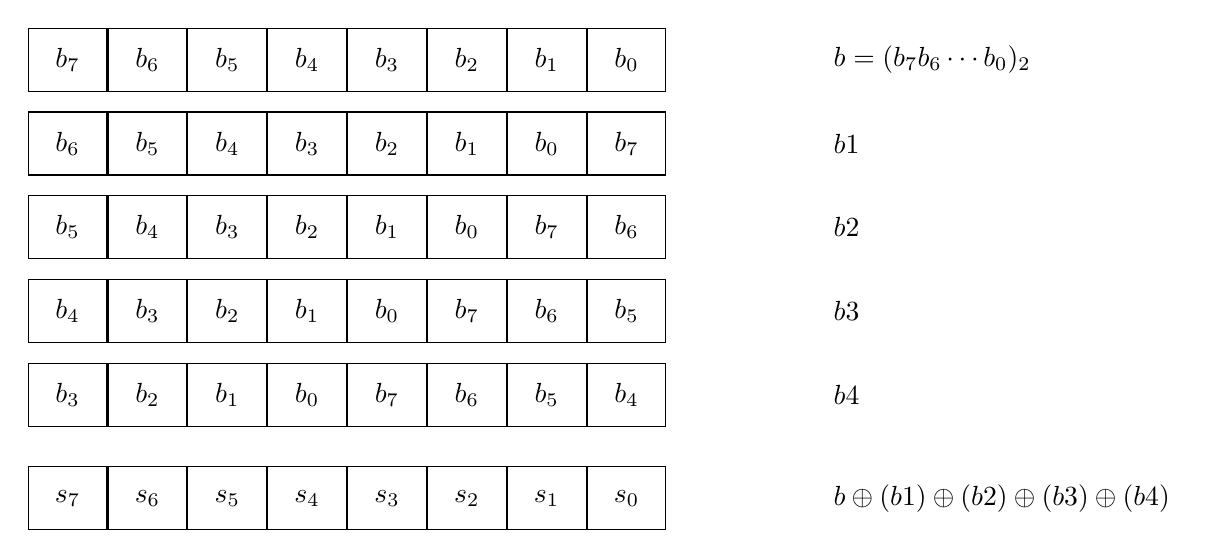
\begin{tikzpicture}[
	box/.style={draw, minimum width=1cm, minimum height=0.8cm, align=center},
	>=latex
	]
	\node[box] (a0) at (0,2) {$b_7$};
	\node[box] (a1) [right=0 of a0] {$b_6$};
	\node[box] (a2) [right=0 of a1] {$b_5$};
	\node[box] (a3) [right=0 of a2] {$b_4$};
	\node[box] (a4) [right=0 of a3] {$b_3$};
	\node[box] (a5) [right=0 of a4] {$b_2$};
	\node[box] (a6) [right=0 of a5] {$b_1$};
	\node[box] (a7) [right=0 of a6] {$b_0$};
	\node[] (a8) [right=2 of a7] {$b=(b_7b_6\cdots b_0)_2$};
	
	\node[box] (b0) [below=.25 of a0] {$b_6$};
	\node[box] (b1) [right=0 of b0] {$b_5$};
	\node[box] (b2) [right=0 of b1] {$b_4$};
	\node[box] (b3) [right=0 of b2] {$b_3$};
	\node[box] (b4) [right=0 of b3] {$b_2$};
	\node[box] (b5) [right=0 of b4] {$b_1$};
	\node[box] (b6) [right=0 of b5] {$b_0$};
	\node[box] (b7) [right=0 of b6] {$b_7$};
	\node[] (b8) [right=2 of b7] {$b\lll 1$};
	
	\node[box] (c0) [below=.25 of b0] {$b_5$};
	\node[box] (c1) [right=0 of c0] {$b_4$};
	\node[box] (c2) [right=0 of c1] {$b_3$};
	\node[box] (c3) [right=0 of c2] {$b_2$};
	\node[box] (c4) [right=0 of c3] {$b_1$};
	\node[box] (c5) [right=0 of c4] {$b_0$};
	\node[box] (c6) [right=0 of c5] {$b_7$};
	\node[box] (c7) [right=0 of c6] {$b_6$};
	\node[] (c8) [right=2 of c7] {$b\lll 2$};
	
	\node[box] (d0) [below=.25 of c0] {$b_4$};
	\node[box] (d1) [right=0 of d0] {$b_3$};
	\node[box] (d2) [right=0 of d1] {$b_2$};
	\node[box] (d3) [right=0 of d2] {$b_1$};
	\node[box] (d4) [right=0 of d3] {$b_0$};
	\node[box] (d5) [right=0 of d4] {$b_7$};
	\node[box] (d6) [right=0 of d5] {$b_6$};
	\node[box] (d7) [right=0 of d6] {$b_5$};
	\node[] (d8) [right=2 of d7] {$b\lll 3$};
	
	\node[box] (e0) [below=.25 of d0] {$b_3$};
	\node[box] (e1) [right=0 of e0] {$b_2$};
	\node[box] (e2) [right=0 of e1] {$b_1$};
	\node[box] (e3) [right=0 of e2] {$b_0$};
	\node[box] (e4) [right=0 of e3] {$b_7$};
	\node[box] (e5) [right=0 of e4] {$b_6$};
	\node[box] (e6) [right=0 of e5] {$b_5$};
	\node[box] (e7) [right=0 of e6] {$b_4$};
	\node[] (e8) [right=2 of e7] {$b\lll 4$};
	
	\node[box] (f0) [below=.5 of e0] {$s_7$};
	\node[box] (f1) [right=0 of f0] {$s_6$};
	\node[box] (f2) [right=0 of f1] {$s_5$};
	\node[box] (f3) [right=0 of f2] {$s_4$};
	\node[box] (f4) [right=0 of f3] {$s_3$};
	\node[box] (f5) [right=0 of f4] {$s_2$};
	\node[box] (f6) [right=0 of f5] {$s_1$};
	\node[box] (f7) [right=0 of f6] {$s_0$};
	\node[] (f8) [right=2 of f7] {$b\oplus (b\lll 1)\oplus (b\lll 2)\oplus (b\lll 3)\oplus (b\lll 4)$};
\end{tikzpicture}
\end{center}

\newpage
\subsection{Hamming Weight and Hamming Distance on \texorpdfstring{$\mathbb{F}_2^8$}{F2^8}}

\begin{definition}[Hamming weight]
	For a vector
	\[
	x = (x_0,x_1,\dots,x_7)^{\mathsf T} \in \mathbb{F}_2^8,
	\]
	the \emph{Hamming weight} of \(x\) is the number of nonzero coordinates:
	\[
	\mathrm{wt}(x)
	:= \bigl|\{\, i \in \{0,\dots,7\} : x_i = 1 \,\}\bigr|.
	\]
\end{definition}

\begin{definition}[Hamming distance]
	For two vectors
	\[
	x = (x_0,\dots,x_7)^{\mathsf T},\quad
	y = (y_0,\dots,y_7)^{\mathsf T} \in \mathbb{F}_2^8,
	\]
	the \emph{Hamming distance} between \(x\) and \(y\) is
	\[
	d_{\mathrm H}(x,y)
	:= \bigl|\{\, i \in \{0,\dots,7\} : x_i \neq y_i \,\}\bigr|.
	\]
\end{definition}

Since we are working over \(\mathbb{F}_2\), we may equivalently write
\[
d_{\mathrm H}(x,y)
= \mathrm{wt}(x \oplus y),
\]
where \(x \oplus y\) denotes componentwise addition in \(\mathbb{F}_2\) (bitwise XOR).

\medskip

\noindent
In particular, for the vector \(b \in \mathbb{F}_2^8\) and its image \(Ab\) under the linear map
with matrix \(A\), the Hamming distance is
\[
d_{\mathrm H}(b, Ab)
= \mathrm{wt}\bigl( b \oplus Ab \bigr).
\]
Likewise, for a cyclic left rotation \(b \lll k\),
\[
d_{\mathrm H}\bigl(b,\, b \lll k\bigr)
= \mathrm{wt}\bigl( b \oplus (b \lll k) \bigr).
\]

\subsection{Concrete Examples of Hamming Distance}

We work in \(\mathbb{F}_2^8\).

\begin{example}[Hamming distance between two arbitrary vectors]
	Let
	\[
	x =
	\begin{bmatrix}
		1\\0\\1\\1\\0\\0\\1\\0
	\end{bmatrix},
	\qquad
	y =
	\begin{bmatrix}
		0\\1\\1\\0\\0\\1\\0\\0
	\end{bmatrix}
	\in \mathbb{F}_2^8.
	\]
	First compute their componentwise sum (XOR) in \(\mathbb{F}_2\):
	\[
	x \oplus y =
	\begin{bmatrix}
		1\oplus 0\\[2pt]
		0\oplus 1\\[2pt]
		1\oplus 1\\[2pt]
		1\oplus 0\\[2pt]
		0\oplus 0\\[2pt]
		0\oplus 1\\[2pt]
		1\oplus 0\\[2pt]
		0\oplus 0
	\end{bmatrix}
	=
	\begin{bmatrix}
		1\\1\\0\\1\\0\\1\\1\\0
	\end{bmatrix}.
	\]
	The Hamming weight of \(x \oplus y\) is the number of \(1\)'s:
	\[
	\mathrm{wt}(x \oplus y)
	= 5.
	\]
	Therefore the Hamming distance between \(x\) and \(y\) is
	\[
	d_{\mathrm H}(x,y)
	= \mathrm{wt}(x \oplus y)
	= 5.
	\]
\end{example}

\begin{example}[Hamming distance between \(b\) and \(Ab\)]
	Consider the matrix
	\[
	A =
	\begin{bmatrix}
		1 & 0 & 0 & 0 & 1 & 1 & 1 & 1 \\
		1 & 1 & 0 & 0 & 0 & 1 & 1 & 1 \\
		1 & 1 & 1 & 0 & 0 & 0 & 1 & 1 \\
		1 & 1 & 1 & 1 & 0 & 0 & 0 & 1 \\
		1 & 1 & 1 & 1 & 1 & 0 & 0 & 0 \\
		0 & 1 & 1 & 1 & 1 & 1 & 0 & 0 \\
		0 & 0 & 1 & 1 & 1 & 1 & 1 & 0 \\
		0 & 0 & 0 & 1 & 1 & 1 & 1 & 1
	\end{bmatrix},
	\]
	and the vector
	\[
	b =
	\begin{bmatrix}
		1\\0\\0\\0\\0\\0\\0\\0
	\end{bmatrix}
	\in \mathbb{F}_2^8.
	\]
	Then
	\[
	Ab = 1 \cdot
	\begin{bmatrix}
		1\\1\\1\\1\\1\\0\\0\\0
	\end{bmatrix}
	=
	\begin{bmatrix}
		1\\1\\1\\1\\1\\0\\0\\0
	\end{bmatrix},
	\]
	since \(b\) selects the first column of \(A\).
	
	Now compute
	\[
	b \oplus Ab =
	\begin{bmatrix}
		1\\0\\0\\0\\0\\0\\0\\0
	\end{bmatrix}
	\oplus
	\begin{bmatrix}
		1\\1\\1\\1\\1\\0\\0\\0
	\end{bmatrix}
	=
	\begin{bmatrix}
		0\\1\\1\\1\\1\\0\\0\\0
	\end{bmatrix}.
	\]
	The Hamming weight is
	\[
	\mathrm{wt}(b \oplus Ab) = 4,
	\]
	hence the Hamming distance between \(b\) and \(Ab\) is
	\[
	d_{\mathrm H}(b, Ab) = 4.
	\]
\end{example}

\newpage
\subsection{Why a Linear Transformation Acts as Diffusion}

In the standard SPN (Substitution--Permutation Network) model, the state is a vector
space over \(\mathbb{F}_2\). For concreteness, let
\[
V := \mathbb{F}_2^n
\]
with the Hamming weight
\[
\mathrm{wt}(x) := \bigl|\{ i : x_i = 1 \}\bigr|,
\]
and the Hamming distance
\[
d_{\mathrm H}(x,y) := \mathrm{wt}(x + y).
\]

\begin{definition}[Linear diffusion layer]
	A linear map \(L : V \to V\), represented by an invertible matrix \(M \in \mathrm{GL}(n,2)\),
	is called a \emph{diffusion layer} if it spreads nonzero inputs so that
	\(\mathrm{wt}(L(x))\) is typically large whenever \(x \neq 0\).
\end{definition}

Intuitively, a change in a small number of input bits should affect many output bits.

\subsubsection*{1. Componentwise view: each output bit mixes many input bits}

Let \(L(x) = Mx\) with \(M = (M_{ij})\). The \(i\)-th output bit is
\[
(L(x))_i = \sum_{j=1}^n M_{ij} x_j \in \mathbb{F}_2.
\]
Thus, row \(i\) of \(M\) determines which input bits influence output bit \(i\):
\[
(L(x))_i = \bigoplus_{j : M_{ij}=1} x_j.
\]

If each row of \(M\) has many \(1\)'s, then each output bit is the XOR of many input bits.
In particular, flipping a single input bit \(x_k\) changes all output bits \(i\) such that
\(M_{ik} = 1\). Therefore, the number of output bits affected by a single-bit change
in position \(k\) is
\[
\mathrm{wt}\bigl( M e_k \bigr),
\]
where \(e_k\) is the \(k\)-th standard basis vector. A good diffusion layer satisfies
\[
\mathrm{wt}(M e_k) \text{ is large for all } k.
\]

\subsubsection*{2. Hamming weight and branch number}

A deeper global measure of diffusion is the \emph{branch number}.

\begin{definition}[Branch number]
	Let \(L(x) = Mx\) be linear on \(\mathbb{F}_2^n\). The branch number of \(L\) is
	\[
	B(L) := \min_{x \in V \setminus \{0\}} \bigl( \mathrm{wt}(x) + \mathrm{wt}(L(x)) \bigr).
	\]
\end{definition}

If \(B(L)\) is large, then for any nonzero input difference \(x\) we cannot have both
\(\mathrm{wt}(x)\) and \(\mathrm{wt}(L(x))\) small at the same time. In other words:
\[
x \neq 0 \;\Longrightarrow\; \mathrm{wt}(x) + \mathrm{wt}(L(x)) \ge B(L).
\]

Cryptographically, this implies:

\begin{itemize}
	\item If the input difference is concentrated in a few bits (small \(\mathrm{wt}(x)\)),
	then the output difference must be spread over many bits (large \(\mathrm{wt}(L(x))\)).
	\item In an SPN with parallel S-boxes, \(L\) acts between nonlinear layers.
	A large branch number forces many S-boxes to become ``active'' in the following
	rounds, which raises the cost of any differential or linear trail.
\end{itemize}

Thus, the branch number is a \emph{purely linear-algebraic} quantity that quantifies
how well the matrix \(M\) performs diffusion.

\subsubsection*{3. Linearity and propagation of differences}

Let \(L(x) = Mx\) be linear and consider two inputs \(x,y \in V\). The difference of outputs is
\[
L(x) + L(y) = L(x+y).
\]
Hence, the evolution of \emph{differences} under \(L\) is exactly the evolution of
single vectors under the same linear map. In particular, if \(\Delta = x+y\), then
\[
\Delta_{\text{out}} = L(x) + L(y) = L(\Delta).
\]

Therefore, the way small input differences spread through the cipher is controlled
entirely by the linear map \(L\) between the nonlinear S-box layers. Good diffusion
means: for all nonzero \(\Delta\), the Hamming weight \(\mathrm{wt}(L(\Delta))\) is large,
and the branch number \(B(L)\) is high.

\subsubsection*{4. Why linear?}

There are several reasons why diffusion is implemented \emph{linearly}:

\begin{itemize}
	\item \textbf{Simplicity and efficiency.} Matrix multiplication over \(\mathbb{F}_2\)
	is easy to implement in both hardware and software (XORs and bit shifts).
	
	\item \textbf{Invariance of nonlinear strength.} Composing a nonlinear S-box with an
	invertible linear map \(L\) (before or after) yields an \emph{affine-equivalent}
	S-box with the same nonlinearity and differential uniformity. Thus one can
	design nonlinearity (via inversion in \(\mathbb{F}_{2^8}\), for instance) and
	diffusion (via a carefully chosen \(M\)) largely independently.
	
	\item \textbf{Clean analysis.} Because \(L\) is linear, its effect on differences (and on
	linear masks) is completely determined by standard linear algebra over
	\(\mathbb{F}_2\). This makes it possible to prove lower bounds on the number
	of active S-boxes in multiple rounds (the ``wide trail'' strategy).
\end{itemize}

\subsubsection*{5. Example: the given \(8\times 8\) matrix}

For the specific matrix
\[
A =
\begin{bmatrix}
	1 & 0 & 0 & 0 & 1 & 1 & 1 & 1 \\
	1 & 1 & 0 & 0 & 0 & 1 & 1 & 1 \\
	1 & 1 & 1 & 0 & 0 & 0 & 1 & 1 \\
	1 & 1 & 1 & 1 & 0 & 0 & 0 & 1 \\
	1 & 1 & 1 & 1 & 1 & 0 & 0 & 0 \\
	0 & 1 & 1 & 1 & 1 & 1 & 0 & 0 \\
	0 & 0 & 1 & 1 & 1 & 1 & 1 & 0 \\
	0 & 0 & 0 & 1 & 1 & 1 & 1 & 1
\end{bmatrix},
\]
we have:

\begin{itemize}
	\item \(A \in \mathrm{GL}(8,2)\): it is invertible over \(\mathbb{F}_2\), so no information is lost.
	\item Each row has \(5\) ones: every output bit is the XOR of \(5\) input bits.
	\item The branch number is
	\[
	B(A) = \min_{x\neq 0} \bigl( \mathrm{wt}(x) + \mathrm{wt}(Ax) \bigr) = 4,
	\]
	so no nonzero difference can remain concentrated in too few bits in both
	input and output simultaneously.
\end{itemize}

These are precisely the linear-algebraic features that make a matrix like \(A\)
serve as a diffusion layer in a cipher: it spreads any local change across many
coordinates and, when iterated between nonlinear layers, forces a large part of
the state to be affected.


\newpage
\subsection{A Geometric Viewpoint in Finite Dimension}

We work over the vector space
\[
V := \mathbb{F}_2^8.
\]
The elements of \(V\) may be viewed as the vertices of the \(8\)-dimensional
Hamming cube. Concretely,
\[
V = \{0,1\}^8,
\]
and we equip \(V\) with the Hamming distance
\[
d(x,y) := \bigl|\{ i \in \{0,\dots,7\} : x_i \neq y_i \}\bigr|.
\]
Two vertices are joined by an edge if and only if they differ in exactly one
coordinate (i.e.\ distance \(1\)).

The linear map associated to the matrix
\[
A =
\begin{bmatrix}
	1 & 0 & 0 & 0 & 1 & 1 & 1 & 1 \\
	1 & 1 & 0 & 0 & 0 & 1 & 1 & 1 \\
	1 & 1 & 1 & 0 & 0 & 0 & 1 & 1 \\
	1 & 1 & 1 & 1 & 0 & 0 & 0 & 1 \\
	1 & 1 & 1 & 1 & 1 & 0 & 0 & 0 \\
	0 & 1 & 1 & 1 & 1 & 1 & 0 & 0 \\
	0 & 0 & 1 & 1 & 1 & 1 & 1 & 0 \\
	0 & 0 & 0 & 1 & 1 & 1 & 1 & 1
\end{bmatrix}
\]
is the map \(T:V \to V\) defined by
\[
T(b) = Ab.
\]
Equivalently, in terms of cyclic left rotations (indices modulo \(8\)),
\[
T(b) = b \oplus (b \lll 1) \oplus (b \lll 2) \oplus (b \lll 3) \oplus (b \lll 4),
\]
so that each coordinate satisfies
\[
(T(b))_i = b_i \oplus b_{i-1} \oplus b_{i-2} \oplus b_{i-3} \oplus b_{i-4}
\quad (i \in \mathbb{Z}_8).
\]

\begin{itemize}
	\item As a linear transformation, \(T\) is a bijection of \(V\), i.e.\
	\(A \in \mathrm{GL}(8,2)\). In geometric terms, \(T\) is an
	\emph{automorphism} of the finite affine space \(\mathrm{AG}(8,2)\).
	
	\item Lines in \(V\) are affine \(1\)-dimensional subspaces of the form
	\(\ell = x + \mathbb{F}_2 v\), where \(v \neq 0\).
	Since \(T\) is linear, it maps lines to lines:
	\[
	T(\ell) = T(x) + \mathbb{F}_2\,T(v).
	\]
	More generally, every affine subspace (finite ``flat'') is mapped to
	an affine subspace of the same dimension.
	
	\item Thus \(T\) preserves the entire incidence structure of the Hamming cube:
	it permutes vertices, carries edges to edges, and maps affine
	\(k\)-dimensional subspaces to affine \(k\)-dimensional subspaces.
	In this sense, \(T\) is a geometric symmetry of the finite space
	\(\mathbb{F}_2^8\).
\end{itemize}

\subsection{Why the Expression \texorpdfstring{$b \oplus (b \lll 1) \oplus (b \lll 2) \oplus (b \lll 3) \oplus (b \lll 4)$}{b xor rotations} Corresponds to the Matrix \(A\)}

We work over the vector space \(\mathbb{F}_2^8\). Let
\[
b =
\begin{bmatrix}
	b_0\\ b_1\\ b_2\\ b_3\\ b_4\\ b_5\\ b_6\\ b_7
\end{bmatrix}
\in \mathbb{F}_2^8,
\]
and interpret the index set \(\{0,1,\dots,7\}\) as the cyclic group \(\mathbb{Z}_8\). Addition of indices is always taken modulo~\(8\).

\begin{definition}[Cyclic left rotation]
	For \(k \in \mathbb{Z}_8\), the cyclic left rotation of \(b\) by \(k\) positions, denoted \(b \lll k\), is the vector \(b' \in \mathbb{F}_2^8\) with
	\[
	(b \lll k)_i := b_{\,i-k}, \qquad i \in \mathbb{Z}_8,
	\]
	where the index \(i-k\) is taken modulo \(8\).
\end{definition}

\noindent
Thus, componentwise, we have
\[
(b \lll 0)_i = b_i,\quad
(b \lll 1)_i = b_{i-1},\quad
(b \lll 2)_i = b_{i-2},\quad
(b \lll 3)_i = b_{i-3},\quad
(b \lll 4)_i = b_{i-4}.
\]

Consider the linear map
\[
T : \mathbb{F}_2^8 \to \mathbb{F}_2^8,\qquad
T(b) := b \oplus (b \lll 1) \oplus (b \lll 2) \oplus (b \lll 3) \oplus (b \lll 4),
\]
where \(\oplus\) denotes addition in \(\mathbb{F}_2\) (bitwise XOR).

\paragraph{Step 1: Coordinate formula for \(T(b)\).}
Let \(c := T(b)\), so \(c = (c_0,\dots,c_7)^{\mathsf T}\). Then for each \(i \in \mathbb{Z}_8\),
\begin{align*}
	c_i
	&= (b)_i \oplus (b \lll 1)_i \oplus (b \lll 2)_i \oplus (b \lll 3)_i \oplus (b \lll 4)_i \\
	&= b_i \oplus b_{i-1} \oplus b_{i-2} \oplus b_{i-3} \oplus b_{i-4}.
\end{align*}
In other words,
\[
c_i = \sum_{k=0}^{4} b_{\,i-k} \quad \text{in } \mathbb{F}_2.
\]

Explicitly, writing out the eight coordinates:
\[
\begin{aligned}
	c_0 &= b_0 \oplus b_7 \oplus b_6 \oplus b_5 \oplus b_4,\\
	c_1 &= b_1 \oplus b_0 \oplus b_7 \oplus b_6 \oplus b_5,\\
	c_2 &= b_2 \oplus b_1 \oplus b_0 \oplus b_7 \oplus b_6,\\
	c_3 &= b_3 \oplus b_2 \oplus b_1 \oplus b_0 \oplus b_7,\\
	c_4 &= b_4 \oplus b_3 \oplus b_2 \oplus b_1 \oplus b_0,\\
	c_5 &= b_5 \oplus b_4 \oplus b_3 \oplus b_2 \oplus b_1,\\
	c_6 &= b_6 \oplus b_5 \oplus b_4 \oplus b_3 \oplus b_2,\\
	c_7 &= b_7 \oplus b_6 \oplus b_5 \oplus b_4 \oplus b_3.
\end{aligned}
\]

\paragraph{Step 2: Read off the matrix entries.}
Let \(A\) denote the matrix of the linear map \(T\) with respect to the standard basis of \(\mathbb{F}_2^8\). By definition, the entries \(A_{i,j}\) satisfy
\[
c_i = (T(b))_i = \sum_{j=0}^{7} A_{i,j} b_j,
\]
with addition in \(\mathbb{F}_2\).

From the coordinate formula
\[
c_i = b_i \oplus b_{i-1} \oplus b_{i-2} \oplus b_{i-3} \oplus b_{i-4},
\]
we see that
\[
A_{i,j} =
\begin{cases}
	1, & \text{if } j \in \{i,\,i-1,\,i-2,\,i-3,\,i-4\} \text{ mod } 8,\\
	0, & \text{otherwise}.
\end{cases}
\]

Writing out the rows explicitly (with indices \(0,\dots,7\) in order), we obtain
\[
A =
\begin{bmatrix}
	1 & 0 & 0 & 0 & 1 & 1 & 1 & 1 \\
	1 & 1 & 0 & 0 & 0 & 1 & 1 & 1 \\
	1 & 1 & 1 & 0 & 0 & 0 & 1 & 1 \\
	1 & 1 & 1 & 1 & 0 & 0 & 0 & 1 \\
	1 & 1 & 1 & 1 & 1 & 0 & 0 & 0 \\
	0 & 1 & 1 & 1 & 1 & 1 & 0 & 0 \\
	0 & 0 & 1 & 1 & 1 & 1 & 1 & 0 \\
	0 & 0 & 0 & 1 & 1 & 1 & 1 & 1
\end{bmatrix}.
\]

\paragraph{Conclusion.}
By construction, for every \(b \in \mathbb{F}_2^8\),
\[
T(b) = b \oplus (b \lll 1) \oplus (b \lll 2) \oplus (b \lll 3) \oplus (b \lll 4)
\]
and
\[
T(b) = Ab.
\]
Therefore, the expression
\[
b \oplus (b \lll 1) \oplus (b \lll 2) \oplus (b \lll 3) \oplus (b \lll 4)
\]
is exactly the action of the matrix \(A\) on the vector \(b\) in the standard basis of \(\mathbb{F}_2^8\).

\newpage
\[
A
\begin{bmatrix}
	b_0\\ b_1\\ b_2\\ b_3\\ b_4\\ b_5\\ b_6\\ b_7
\end{bmatrix}
=
b_0
\begin{bmatrix}
	1\\ 1\\ 1\\ 1\\ 1\\ 0\\ 0\\ 0
\end{bmatrix}
+
b_1
\begin{bmatrix}
	0\\ 1\\ 1\\ 1\\ 1\\ 1\\ 0\\ 0
\end{bmatrix}
+
b_2
\begin{bmatrix}
	0\\ 0\\ 1\\ 1\\ 1\\ 1\\ 1\\ 0
\end{bmatrix}
+
b_3
\begin{bmatrix}
	0\\ 0\\ 0\\ 1\\ 1\\ 1\\ 1\\ 1
\end{bmatrix}
+
b_4
\begin{bmatrix}
	1\\ 0\\ 0\\ 0\\ 1\\ 1\\ 1\\ 1
\end{bmatrix}
+
b_5
\begin{bmatrix}
	1\\ 1\\ 0\\ 0\\ 0\\ 1\\ 1\\ 1
\end{bmatrix}
+
b_6
\begin{bmatrix}
	1\\ 1\\ 1\\ 0\\ 0\\ 0\\ 1\\ 1
\end{bmatrix}
+
b_7
\begin{bmatrix}
	1\\ 1\\ 1\\ 1\\ 0\\ 0\\ 0\\ 1
\end{bmatrix}.
\]

We write
\[
b =
\begin{bmatrix}
	b_0\\ b_1\\ b_2\\ b_3\\ b_4\\ b_5\\ b_6\\ b_7
\end{bmatrix}
\in \mathbb{F}_2^8.
\]
Then each coordinate of \(Ab\) is a linear combination of \(\{b_0,\dots,b_7\}\) with coefficients in \(\mathbb{F}_2\):

\[
Ab =
\begin{bmatrix}
	c_0\\ c_1\\ c_2\\ c_3\\ c_4\\ c_5\\ c_6\\ c_7
\end{bmatrix}
=
\begin{bmatrix}
	b_0 + b_4 + b_5 + b_6 + b_7 \\
	b_0 + b_1 + b_5 + b_6 + b_7 \\
	b_0 + b_1 + b_2 + b_6 + b_7 \\
	b_0 + b_1 + b_2 + b_3 + b_7 \\
	b_0 + b_1 + b_2 + b_3 + b_4 \\
	b_1 + b_2 + b_3 + b_4 + b_5 \\
	b_2 + b_3 + b_4 + b_5 + b_6 \\
	b_3 + b_4 + b_5 + b_6 + b_7
\end{bmatrix}.
\]

Equivalently, in compact index notation (indices taken modulo \(8\)),
\[
(Ab)_i = \sum_{k=0}^{4} b_{\,i-k}
\quad\text{for } i = 0,1,\dots,7,
\]
so every entry \((Ab)_i\) is a linear combination of the scalars \(b_0,\dots,b_7\) with coefficients in \(\{0,1\}\subset\mathbb{F}_2\).

\subsection{Bitwise Description via Cyclic Left Rotations}

Let
\[
b =
\begin{bmatrix}
	b_0\\ b_1\\ b_2\\ b_3\\ b_4\\ b_5\\ b_6\\ b_7
\end{bmatrix}
\in \mathbb{F}_2^8.
\]
We interpret \(b\) as an 8-bit word, where \(b_i\) is the bit in position \(i\), with indices taken in
\(\mathbb{Z}_8 = \{0,1,\dots,7\}\).

\begin{definition}[Cyclic left rotation]
	For \(k \in \mathbb{Z}_8\), the \emph{cyclic left rotation} of \(b\) by \(k\) bits, denoted
	\(b \lll k\), is the vector in \(\mathbb{F}_2^8\) whose \(i\)-th component is
	\[
	(b \lll k)_i := b_{\,i-k \bmod 8}, \qquad i \in \mathbb{Z}_8.
	\]
\end{definition}

With this convention, the matrix
\[
A =
\begin{bmatrix}
	1 & 0 & 0 & 0 & 1 & 1 & 1 & 1 \\
	1 & 1 & 0 & 0 & 0 & 1 & 1 & 1 \\
	1 & 1 & 1 & 0 & 0 & 0 & 1 & 1 \\
	1 & 1 & 1 & 1 & 0 & 0 & 0 & 1 \\
	1 & 1 & 1 & 1 & 1 & 0 & 0 & 0 \\
	0 & 1 & 1 & 1 & 1 & 1 & 0 & 0 \\
	0 & 0 & 1 & 1 & 1 & 1 & 1 & 0 \\
	0 & 0 & 0 & 1 & 1 & 1 & 1 & 1
\end{bmatrix}
\]
acts on \(b\) by
\[
Ab =
\begin{bmatrix}
	b_0 + b_4 + b_5 + b_6 + b_7 \\
	b_0 + b_1 + b_5 + b_6 + b_7 \\
	b_0 + b_1 + b_2 + b_6 + b_7 \\
	b_0 + b_1 + b_2 + b_3 + b_7 \\
	b_0 + b_1 + b_2 + b_3 + b_4 \\
	b_1 + b_2 + b_3 + b_4 + b_5 \\
	b_2 + b_3 + b_4 + b_5 + b_6 \\
	b_3 + b_4 + b_5 + b_6 + b_7
\end{bmatrix},
\]
where addition is in \(\mathbb{F}_2\) (bitwise XOR).

Equivalently, each component satisfies
\[
(Ab)_i
= b_i + b_{i-1} + b_{i-2} + b_{i-3} + b_{i-4}
\quad\text{for all } i \in \mathbb{Z}_8,
\]
so that
\[
Ab
= b \oplus (b \lll 1) \oplus (b \lll 2) \oplus (b \lll 3) \oplus (b \lll 4),
\]
where \(\oplus\) denotes bitwise XOR and \(\lll k\) is 8-bit cyclic left rotation by \(k\) positions.


\newpage
\section{Computing \texorpdfstring{$Ab$}{Ab} in Several Ways}

We consider the matrix
\[
A =
\begin{bmatrix}
	1 & 0 & 0 & 0 & 1 & 1 & 1 & 1 \\
	1 & 1 & 0 & 0 & 0 & 1 & 1 & 1 \\
	1 & 1 & 1 & 0 & 0 & 0 & 1 & 1 \\
	1 & 1 & 1 & 1 & 0 & 0 & 0 & 1 \\
	1 & 1 & 1 & 1 & 1 & 0 & 0 & 0 \\
	0 & 1 & 1 & 1 & 1 & 1 & 0 & 0 \\
	0 & 0 & 1 & 1 & 1 & 1 & 1 & 0 \\
	0 & 0 & 0 & 1 & 1 & 1 & 1 & 1
\end{bmatrix}
\]
and the column vector
\[
b =
\begin{bmatrix}
	b_0\\ b_1\\ b_2\\ b_3\\ b_4\\ b_5\\ b_6\\ b_7
\end{bmatrix}.
\]
We write
\[
Ab =
\begin{bmatrix}
	c_0\\ c_1\\ c_2\\ c_3\\ c_4\\ c_5\\ c_6\\ c_7
\end{bmatrix}.
\]

\subsection{Direct Row-by-Row Computation}

Each component \(c_i\) is the dot product of the \(i\)-th row of \(A\) with the vector \(b\). Thus
\[
\begin{aligned}
	c_0 &= b_0 + b_4 + b_5 + b_6 + b_7,\\
	c_1 &= b_0 + b_1 + b_5 + b_6 + b_7,\\
	c_2 &= b_0 + b_1 + b_2 + b_6 + b_7,\\
	c_3 &= b_0 + b_1 + b_2 + b_3 + b_7,\\
	c_4 &= b_0 + b_1 + b_2 + b_3 + b_4,\\
	c_5 &= b_1 + b_2 + b_3 + b_4 + b_5,\\
	c_6 &= b_2 + b_3 + b_4 + b_5 + b_6,\\
	c_7 &= b_3 + b_4 + b_5 + b_6 + b_7.
\end{aligned}
\]
Here the addition can be understood either as ordinary addition (over \(\mathbb{R}\)) or as addition in \(\mathbb{F}_2\) (bitwise XOR).

In vector form,
\[
Ab =
\begin{bmatrix}
	b_0 + b_4 + b_5 + b_6 + b_7 \\
	b_0 + b_1 + b_5 + b_6 + b_7 \\
	b_0 + b_1 + b_2 + b_6 + b_7 \\
	b_0 + b_1 + b_2 + b_3 + b_7 \\
	b_0 + b_1 + b_2 + b_3 + b_4 \\
	b_1 + b_2 + b_3 + b_4 + b_5 \\
	b_2 + b_3 + b_4 + b_5 + b_6 \\
	b_3 + b_4 + b_5 + b_6 + b_7
\end{bmatrix}.
\]

\subsection{Interpretation over \texorpdfstring{$\mathbb{F}_2$}{F2} (XOR Form)}

If \(b_i \in \{0,1\}\) and we work over the field \(\mathbb{F}_2\), we usually write \(\oplus\) for addition (XOR). Then
\[
\begin{aligned}
	c_0 &= b_0 \oplus b_4 \oplus b_5 \oplus b_6 \oplus b_7,\\
	c_1 &= b_0 \oplus b_1 \oplus b_5 \oplus b_6 \oplus b_7,\\
	c_2 &= b_0 \oplus b_1 \oplus b_2 \oplus b_6 \oplus b_7,\\
	c_3 &= b_0 \oplus b_1 \oplus b_2 \oplus b_3 \oplus b_7,\\
	c_4 &= b_0 \oplus b_1 \oplus b_2 \oplus b_3 \oplus b_4,\\
	c_5 &= b_1 \oplus b_2 \oplus b_3 \oplus b_4 \oplus b_5,\\
	c_6 &= b_2 \oplus b_3 \oplus b_4 \oplus b_5 \oplus b_6,\\
	c_7 &= b_3 \oplus b_4 \oplus b_5 \oplus b_6 \oplus b_7.
\end{aligned}
\]

\subsection{Cyclic Convolution Description}

Let the indices be taken modulo \(8\), i.e.\ we regard \(\{0,1,\dots,7\}\) as \(\mathbb{Z}_8\). Then each output component \(c_i\) is a sum of five consecutive inputs:
\[
c_i = \sum_{k=0}^{4} b_{\,i-k \bmod 8}, \qquad i \in \{0,1,\dots,7\}.
\]
In other words, the linear map \(b \mapsto Ab\) is the \emph{circular convolution} of the sequence
\[
(b_0,b_1,\dots,b_7)
\]
with the \emph{kernel}
\[
h = (1,1,1,1,1,0,0,0).
\]

\subsection{Polynomial Representation in \texorpdfstring{$\mathbb{F}_2[x]/(x^8-1)$}{F2[x]/(x8-1)}}

Encode the vector \(b\) as a polynomial
\[
B(x) = b_0 + b_1 x + b_2 x^2 + \cdots + b_7 x^7
\]
with coefficients in \(\mathbb{F}_2\). Define
\[
H(x) = 1 + x + x^2 + x^3 + x^4.
\]
Then the product \(Ab\) corresponds to the polynomial
\[
C(x) = H(x)\,B(x) \bmod (x^8 - 1),
\]
and the coefficients of \(C(x)\) are precisely the components \(c_0,\dots,c_7\) of the vector \(Ab\).

Thus the single matrix--vector product
\[
Ab
\]
admits equivalent descriptions as:
\begin{itemize}
	\item an explicit linear combination of the \(b_i\),
	\item a bitwise XOR of selected coordinates (over \(\mathbb{F}_2\)),
	\item a cyclic convolution with the kernel \((1,1,1,1,1,0,0,0)\),
	\item multiplication by \(1 + x + x^2 + x^3 + x^4\) in the quotient ring \(\mathbb{F}_2[x]/(x^8 - 1)\).
\end{itemize}

\newpage
\section{The Ambient Vector Space}

We work throughout over the finite field
\[
\F_2 = \{0,1\}
\]
with addition and multiplication taken modulo \(2\).

\begin{definition}
	Let
	\[
	V := \F_2^8
	\]
	denote the \(8\)-dimensional vector space of column vectors with entries in \(\F_2\). An element
	\[
	x \in V
	\]
	is a column vector
	\[
	x = \begin{pmatrix} x_0\\x_1\\\vdots\\x_7\end{pmatrix}, \quad x_i \in \F_2,
	\]
	with addition and scalar multiplication defined componentwise over \(\F_2\).
\end{definition}

\begin{definition}
	The \emph{standard basis} of \(V\) is the family
	\[
	e_i = \begin{pmatrix}0\\\vdots\\1\\\vdots\\0\end{pmatrix}, 
	\quad i = 0,\dots,7,
	\]
	where the entry \(1\) is in position \(i\) and all other entries are \(0\).
\end{definition}

Every \(x \in V\) has a unique representation
\[
x = \sum_{i=0}^7 x_i e_i.
\]

\section{Linear Maps and Invertibility}

\begin{definition}
	A map \(L : V \to V\) is called \emph{linear} if for all \(x,y \in V\) and all \(\alpha,\beta \in \F_2\),
	\[
	L(\alpha x + \beta y) = \alpha L(x) + \beta L(y).
	\]
\end{definition}

With respect to the standard basis of \(V\), every linear map \(L\) is represented by a unique matrix
\[
M \in \Mat_{8 \times 8}(\F_2)
\]
such that
\[
L(x) = Mx
\]
for all \(x \in V\).

\begin{definition}
	A linear map \(L : V \to V\) is called \emph{invertible} if there exists a linear map \(L^{-1} : V \to V\) such that
	\[
	L^{-1} \circ L = \id_V
	\quad\text{and}\quad
	L \circ L^{-1} = \id_V.
	\]
\end{definition}

\begin{lemma}\label{lem:invertible-matrix-equivalences}
	Let \(M \in \Mat_{8\times 8}(\F_2)\). The following are equivalent:
	\begin{enumerate}
		\item The map \(x \mapsto Mx\) is invertible as a linear map \(V \to V\).
		\item \(\ker(M) = \{0\}\).
		\item \(\rankop(M) = 8\).
		\item \(\detop(M) = 1 \in \F_2\).
	\end{enumerate}
\end{lemma}

\noindent
The group of invertible \(8\times 8\) matrices over \(\F_2\) is denoted
\[
\GL(8,2) := \{ M \in \Mat_{8 \times 8}(\F_2) : \detop(M) = 1 \}.
\]

\section{Affine Transformations of \texorpdfstring{\(V\)}{V}}

\begin{definition}
	A map \(A : V \to V\) is called \emph{affine} if there exists a linear map \(L : V \to V\) and a vector \(c \in V\) such that
	\[
	A(x) = L(x) + c \quad \text{for all } x \in V.
	\]
	The linear map \(L\) is called the \emph{linear part} of \(A\).
\end{definition}

In coordinates, if \(L(x) = Mx\) for some \(M \in \Mat_{8 \times 8}(\F_2)\), then
\[
A(x) = Mx + c, \quad c \in V.
\]

\begin{proposition}\label{prop:invertible-affine}
	Let \(A : V \to V\) be given by
	\[
	A(x) = Mx + c
	\]
	with \(M \in \Mat_{8 \times 8}(\F_2)\) and \(c \in V\). Then
	\[
	A \text{ is bijective } \Longleftrightarrow M \in \GL(8,2).
	\]
\end{proposition}

\begin{proof}
	Suppose first that \(M \in \GL(8,2)\). Then we define a map \(A^{-1} : V \to V\) by
	\[
	A^{-1}(y) := M^{-1} (y - c).
	\]
	This is well-defined and affine. For all \(x \in V\),
	\[
	A^{-1}(A(x)) 
	= M^{-1} (Mx + c - c) 
	= M^{-1} Mx 
	= x,
	\]
	and for all \(y \in V\),
	\[
	A(A^{-1}(y))
	= M \bigl( M^{-1} (y - c) \bigr) + c
	= (y - c) + c
	= y.
	\]
	Thus \(A\) is bijective.
	
	Conversely, suppose \(A\) is bijective. Let \(x,x' \in V\) satisfy \(M x = M x'\). Then
	\[
	A(x) - c = Mx = Mx' = A(x') - c,
	\]
	so \(A(x) = A(x')\). By injectivity of \(A\), it follows that \(x = x'\). Hence the linear map \(x \mapsto Mx\) is injective and thus invertible. Therefore \(M \in \GL(8,2)\).
\end{proof}

\section{The Rijndael S-Box as a Composition}

\subsection{The Nonlinear Core}

The Rijndael (AES) S-box is a permutation
\[
S : V \to V
\]
constructed as the composition of two conceptually distinct steps:
\begin{enumerate}
	\item a nonlinear permutation \(N : V \to V\), and
	\item an affine transformation \(A_{\mathrm{aff}}(x) = Mx + c\), with \(M \in \GL(8,2)\), \(c \in V\).
\end{enumerate}

To define \(N\), one first identifies \(V\) with the finite field \(\F_{2^8}\) via a fixed \(\F_2\)-vector-space isomorphism
\[
\varphi : \F_{2^8} \to V.
\]

\begin{definition}
	Define a permutation \(N : V \to V\) by
	\[
	N(x) = 
	\begin{cases}
		\varphi\bigl( (\varphi^{-1}(x))^{-1} \bigr), & \text{if } x \neq 0,\\[4pt]
		0, & \text{if } x = 0.
	\end{cases}
	\]
\end{definition}

The map \(N\) is the multiplicative inverse on \(\F_{2^8}\), expressed in the coordinate representation \(V\). It is not linear over \(\F_2\).

\subsection{Affine Output Transformation}

The Rijndael S-box is then defined by
\[
S(x) := M \cdot N(x) + c,
\]
where \(M \in \GL(8,2)\) and \(c \in V\) are fixed. By Proposition~\ref{prop:invertible-affine} and the fact that \(N\) is a permutation, we see that \(S\) is a permutation:
\[
S = A_{\mathrm{aff}} \circ N,
\]
and the composition of two bijections is a bijection.

From a linear algebraic perspective, once the nonlinear permutation \(N\) is fixed, the S-box is determined entirely by the choice of the pair \((M,c)\), with \(M \in \GL(8,2)\).

\section{Linear-Algebraic Notions of Diffusion}

\subsection{Hamming Weight and Bit Diffusion}

\begin{definition}
	For \(x = (x_0,\dots,x_7)^{\mathsf{T}} \in V\), the \emph{Hamming weight} of \(x\) is the integer
	\[
	\wt(x) := \left| \{ i \in \{0,\dots,7\} : x_i = 1 \} \right|.
	\]
\end{definition}

\begin{definition}
	Let \(L : V \to V\) be linear, \(L(x) = Mx\). We say that \(L\) has good \emph{bit-wise diffusion} if:
	\begin{enumerate}
		\item For every nonzero standard basis vector \(e_i\), the weight \(\wt(L(e_i))\) is relatively large.
		\item For every nonzero \(x \in V\), the weight \(\wt(L(x))\) is bounded below by a prescribed constant.
	\end{enumerate}
\end{definition}

The above conditions depend only on the matrix \(M\) and are purely linear in nature.

\subsection{Difference Propagation Through the Affine Layer}

Let \(S(x) = M N(x) + c\) be the S-box. For any \(\Delta x \in V\) and all \(x \in V\),
\begin{align*}
	S(x + \Delta x) + S(x)
	&= M N(x + \Delta x) + c + M N(x) + c \\
	&= M \bigl( N(x + \Delta x) + N(x) \bigr).
\end{align*}
Thus the difference
\[
\Delta S := S(x + \Delta x) + S(x)
\]
is obtained by applying the linear map \(M\) to the \emph{nonlinear difference}
\[
\Delta N := N(x + \Delta x) + N(x).
\]

\begin{lemma}
	For all \(x,\Delta x \in V\),
	\[
	S(x + \Delta x) + S(x) = M\bigl( N(x + \Delta x) + N(x) \bigr).
	\]
	In particular, the mapping \(\Delta N \mapsto \Delta S\) is entirely determined by the linear map \(M\).
\end{lemma}

\subsection{Branch Number}

\begin{definition}
	Let \(L : V \to V\) be linear, \(L(x) = Mx\). The \emph{branch number} of \(L\) is defined as
	\[
	B(L) := \min_{x \in V \setminus \{0\}} \bigl( \wt(x) + \wt(L(x)) \bigr).
	\]
\end{definition}

A large branch number means that for every nonzero \(x\), it is impossible for both \(x\) and \(L(x)\) to have simultaneously small Hamming weight. This is a purely linear property of the matrix \(M\).

In the context of the S-box, once the nonlinear part \(N\) is fixed, the branch number of the affine layer \(L(x) = Mx\) is a fundamental linear-algebraic measure of how effectively bit patterns are spread.

\section{Affine Transformations and Change of Basis}

\subsection{Change of Basis in \texorpdfstring{\(V\)}{V}}

Let \(\mathcal{B} = \{b_0,\dots,b_7\}\) be a basis of \(V\). Every \(x \in V\) can be written uniquely as
\[
x = \sum_{i=0}^7 \alpha_i b_i, \quad \alpha_i \in \F_2.
\]
We define the coordinate column vector of \(x\) with respect to \(\mathcal{B}\) as
\[
[x]_{\mathcal{B}} 
:= \begin{pmatrix} \alpha_0\\\vdots\\\alpha_7 \end{pmatrix} \in V.
\]

If \(\mathcal{B}' = \{b'_0,\dots,b'_7\}\) is another basis, then there exists a unique matrix \(P \in \GL(8,2)\) such that
\[
[x]_{\mathcal{B}'} = P\, [x]_{\mathcal{B}}
\]
for all \(x \in V\). Thus every change of basis in \(V\) is represented by left-multiplication by an element of \(\GL(8,2)\).

\subsection{Conjugation of the Nonlinear Core}

Let \(N : V \to V\) be the nonlinear permutation induced by inversion in \(\F_{2^8}\), as defined earlier. If we change coordinates by a matrix \(P \in \GL(8,2)\), then the coordinate representation of \(N\) in the new basis is the conjugate map
\[
N'(x) := P\, N(P^{-1} x).
\]

Thus composing \(N\) with invertible linear maps on the left and right corresponds to viewing the same abstract permutation under different coordinate systems.

The affine post-transformation used in the Rijndael S-box,
\[
A_{\mathrm{aff}}(x) = Mx + c,
\]
is therefore not merely an implementational detail: its linear part \(M\) selects a particular way of mixing the coordinates of the output of the nonlinear core \(N\) before presenting them as the final S-box output bits.

\section{Linear-Algebraic Constraints on the Rijndael Matrix}

From a purely linear algebraic point of view, the choice of the Rijndael S-box matrix \(M\) can be described as the selection of an element of \(\GL(8,2)\) subject to certain constraints. Typical such constraints include:

\begin{enumerate}
	\item \textbf{Invertibility.} One requires
	\[
	M \in \GL(8,2),
	\]
	i.e.\ \(\detop(M) = 1\) in \(\F_2\). By Proposition~\ref{prop:invertible-affine}, this ensures that the affine map \(x \mapsto Mx + c\) is bijective, hence preserves the permutation property of the S-box.
	
	\item \textbf{Non-degenerate bit influence.} For each standard basis vector \(e_i\),
	\[
	\wt(Me_i)
	\]
	should be relatively large, so that changing a single input bit (after the nonlinear map \(N\)) influences many of the output bits of the affine layer.
	
	\item \textbf{Absence of trivial linear relations.} One typically requires that certain subsets of rows or columns of \(M\) are linearly independent, or that submatrices of \(M\) have sufficiently large rank, in order to avoid simple linear relations among output bits in terms of a small number of input bits.
	
	\item \textbf{Good branch number.} One seeks to maximize
	\[
	B(M) := \min_{x \in V \setminus \{0\}} \bigl( \wt(x) + \wt(Mx) \bigr),
	\]
	subject to the above constraints and to implementational considerations. This ensures that any nontrivial input pattern to the affine layer yields an output pattern whose sparsity cannot be simultaneously small.
\end{enumerate}

All of these constraints are expressed purely in terms of linear algebra over \(\F_2\) and are independent of the cryptanalytic details of the nonlinear part \(N\).

\section{The Importance of the \texorpdfstring{\(8 \times 8\)}{8x8} Matrix}

From a linear algebraic perspective, the Rijndael S-box
\[
S(x) = M N(x) + c
\]
is determined, once the nonlinear permutation \(N\) is fixed, by the choice of a single pair \((M,c)\) with \(M \in \GL(8,2)\), \(c \in V\). Among these, the constant vector \(c\) serves to translate all outputs uniformly, while the matrix \(M\) governs the structural properties of the S-box that are visible at the level of linear algebra. Concretely:

\begin{itemize}
	\item \emph{Affine structure.} Every affine map \(A_{\mathrm{aff}} : V \to V\) has the form \(A_{\mathrm{aff}}(x) = Mx + c\). Up to translation, the entire affine structure is captured by the single matrix \(M\).
	
	\item \emph{Bijectivity.} The condition \(M \in \GL(8,2)\), equivalently \(\detop(M) = 1\), is necessary and sufficient for the S-box to remain a permutation, since \(N\) is bijective.
	
	\item \emph{Diffusion.} For any difference \(\Delta x \in V\),
	\[
	S(x + \Delta x) + S(x) = M\bigl( N(x + \Delta x) + N(x) \bigr),
	\]
	so the propagation of differences through the affine layer---as measured, for example, by Hamming weight or branch number---is entirely governed by the linear map \(M\).
	
	\item \emph{Coordinate system.} Since \(\GL(8,2)\) acts as the group of changes of basis on \(V\), the choice of \(M\) specifies a particular coordinate system in which the outputs of \(N\) are expressed. In this sense, \(M\) encodes a distinguished way of mixing and presenting the eight coordinate bits after the nonlinear step.
\end{itemize}

In summary, from a purely linear algebraic standpoint, the Rijndael S-box is the composition of a fixed nonlinear permutation \(N\) with an affine transformation whose linear part is a carefully chosen element \(M \in \GL(8,2)\). All of the structural, coordinate-based properties of the S-box that can be articulated in linear algebraic terms---such as invertibility, diffusion, absence of simple linear relations, and behavior of Hamming weights---are encoded in this single \(8\times 8\) matrix.


\newpage
\section{A Structured \(8\times 8\) Binary Matrix}

We consider the \(8 \times 8\) matrix
\[
M :=
\begin{bmatrix}
	0 & 0 & 1 & 0 & 0 & 1 & 0 & 1 \\
	1 & 0 & 0 & 1 & 0 & 0 & 1 & 0 \\
	0 & 1 & 0 & 0 & 1 & 0 & 0 & 1 \\
	1 & 0 & 1 & 0 & 0 & 1 & 0 & 0 \\
	0 & 1 & 0 & 1 & 0 & 0 & 1 & 0 \\
	0 & 0 & 1 & 0 & 1 & 0 & 0 & 1 \\
	1 & 0 & 0 & 1 & 0 & 1 & 0 & 0 \\
	0 & 1 & 0 & 0 & 1 & 0 & 1 & 0
\end{bmatrix}.
\]

All entries of \(M\) lie in \(\{0,1\}\). Thus \(M\) may be regarded:

\begin{itemize}
	\item either as a matrix with real entries, \(M \in \Mat_{8\times 8}(\mathbb{R})\),
	\item or as a matrix with entries in the finite field \(\mathbb{F}_2\),
	\(M \in \Mat_{8\times 8}(\mathbb{F}_2)\).
\end{itemize}

In both cases, \(M\) defines a linear operator on an \(8\)-dimensional vector space by left multiplication.

\subsection{As a Linear Operator on \(\mathbb{K}^8\)}

Let \(\mathbb{K}\) be a field, and consider the vector space
\[
V := \mathbb{K}^8
\]
of column vectors of length \(8\) over \(\mathbb{K}\). We equip \(V\) with its standard basis
\[
e_1 = \begin{bmatrix}1\\0\\0\\0\\0\\0\\0\\0\end{bmatrix},\;
e_2 = \begin{bmatrix}0\\1\\0\\0\\0\\0\\0\\0\end{bmatrix},\;
\dots,\;
e_8 = \begin{bmatrix}0\\0\\0\\0\\0\\0\\0\\1\end{bmatrix}.
\]

\begin{definition}
	Define the linear operator
	\[
	T : V \to V, \qquad T(x) := Mx.
	\]
\end{definition}

With respect to the standard basis \(\{e_1,\dots,e_8\}\), the matrix of \(T\) is precisely \(M\). The \(j\)-th column of \(M\) is the coordinate vector of \(T(e_j)\):
\[
T(e_j) = M e_j = \text{the \(j\)-th column of }M, \quad j=1,\dots,8.
\]

\subsection{Row and Column Structure}

Each row of \(M\) contains exactly three entries equal to \(1\) and five entries equal to \(0\). Concretely, if we denote by \(\mathbf{1}\) the all-ones column vector
\[
\mathbf{1} :=
\begin{bmatrix}
	1\\1\\1\\1\\1\\1\\1\\1
\end{bmatrix} \in V,
\]
then a direct computation shows that over \(\mathbb{R}\)
\[
M\mathbf{1} =
\begin{bmatrix}
	3\\3\\3\\3\\3\\3\\3\\3
\end{bmatrix}
= 3\,\mathbf{1},
\]
and for every row \(i\),
\[
\sum_{j=1}^{8} M_{ij} = 3.
\]

Similarly, each column of \(M\) has exactly three entries equal to \(1\), so
\[
\sum_{i=1}^{8} M_{ij} = 3 \quad \text{for all } j=1,\dots,8.
\]
In particular, the in-degree and out-degree (see the graph interpretation below) are both equal to \(3\) for every index.

\subsection{Invertibility and Rank}

We now record basic invariants of \(M\).

\begin{proposition}
	Viewed as a matrix over \(\mathbb{R}\), \(M\) has full rank:
	\[
	\rank(M) = 8,
	\]
	and
	\[
	\det(M) = -3 \neq 0.
	\]
	In particular, \(M\) is invertible in \(\Mat_{8\times 8}(\mathbb{R})\), and \(T\) is a linear automorphism of \(\mathbb{R}^8\).
\end{proposition}

\begin{proof}
	A direct computation (for example, by Gaussian elimination or with a computer algebra system) shows that the rows of \(M\) are linearly independent over \(\mathbb{R}\). Thus \(\rank(M)=8\), which forces \(\det(M)\neq 0\). An explicit determinant computation yields \(\det(M)=-3\).
\end{proof}

\begin{corollary}
	Viewed as a matrix over \(\mathbb{F}_2\), one has
	\[
	\det(M) \equiv -3 \equiv 1 \pmod{2},
	\]
	so \(M\) is also invertible in \(\Mat_{8\times 8}(\mathbb{F}_2)\). Hence \(M\) defines an automorphism of the \(8\)-dimensional vector space \(\mathbb{F}_2^8\):
	\[
	M \in \GL(8,2).
	\]
\end{corollary}

\subsection{Spectral Properties Over \(\mathbb{R}\) and \(\mathbb{C}\)}

Over \(\mathbb{R}\) (or \(\mathbb{C}\)), the characteristic polynomial of \(M\) is
\[
\chi_M(x)
= \det(xI_8 - M)
= x^8 - 8x^5 - 38x^4 - 48x^3 - 24x^2 - 8x - 3.
\]
This polynomial factors as
\[
\chi_M(x) = (x - 3)(x + 1)^3\bigl(x^4 + 6x^2 + 1\bigr).
\]

\begin{proposition}
	The eigenvalues of \(M\) over \(\mathbb{C}\) are:
	\[
	\lambda_1 = 3,\quad
	\lambda_2 = -1 \text{ (with algebraic multiplicity \(3\))},
	\]
	and the four roots of
	\[
	x^4 + 6x^2 + 1 = 0,
	\]
	which are purely complex conjugate pairs. The spectral radius of \(M\) is
	\[
	\rho(M) = 3.
	\]
\end{proposition}

\begin{proof}[Proof (sketch)]
	The factorization of \(\chi_M(x)\) follows from a direct computation of \(\det(xI_8 - M)\). The eigenvalues are precisely the roots of \(\chi_M(x)\), with algebraic multiplicities given by the exponents of the linear factors in the factorization. The spectral radius is the maximum of the absolute values of the eigenvalues, which is \(|3|=3\).
\end{proof}

The vector \(\mathbf{1}\) is an eigenvector for the eigenvalue \(3\), since
\[
M\mathbf{1} = 3\mathbf{1}.
\]
A computation of the dimensions of the eigenspaces shows that the geometric multiplicities match the algebraic multiplicities for all eigenvalues, so we obtain:

\begin{proposition}
	Over \(\mathbb{C}\), the matrix \(M\) is diagonalizable. That is, there exists an invertible matrix \(P \in \GL(8,\mathbb{C})\) such that
	\[
	P^{-1} M P = \operatorname{diag}(\lambda_1,\dots,\lambda_8),
	\]
	where \(\lambda_1,\dots,\lambda_8\) are the eigenvalues of \(M\) (listed with multiplicity).
\end{proposition}

Equivalently, the minimal polynomial of \(M\) over \(\mathbb{C}\) is
\[
\mu_M(x) = (x - 3)(x + 1)\bigl(x^4 + 6x^2 + 1\bigr),
\]
each irreducible factor appearing with exponent \(1\).

\subsection{Eigenstructure Over \(\mathbb{F}_2\)}

Over the field \(\mathbb{F}_2\), one can view \(M\) as a linear automorphism of \(\mathbb{F}_2^8\). For example, the all-ones vector
\[
\mathbf{1} =
\begin{bmatrix}
	1\\1\\1\\1\\1\\1\\1\\1
\end{bmatrix}
\in \mathbb{F}_2^8
\]
satisfies
\[
M\mathbf{1}
=
\begin{bmatrix}
	3\\3\\3\\3\\3\\3\\3\\3
\end{bmatrix}
\equiv
\begin{bmatrix}
	1\\1\\1\\1\\1\\1\\1\\1
\end{bmatrix}
\pmod{2},
\]
so \(\mathbf{1}\) is an eigenvector with eigenvalue \(1 \in \mathbb{F}_2\). Thus \(\mathbf{1}\) spans a one-dimensional invariant subspace of \(\mathbb{F}_2^8\) under \(M\).

More generally, one may study the Jordan normal form of \(M\) over an algebraic closure of \(\mathbb{F}_2\), or equivalently the factorization of \(\chi_M(x)\) modulo \(2\). This describes the cycle structure of the permutation induced by \(M\) on the nonzero vectors of \(\mathbb{F}_2^8\).

\subsection{Graph-Theoretic Interpretation}

Because all entries of \(M\) are \(0\) or \(1\), the matrix \(M\) can be interpreted as the adjacency matrix of a directed graph on the vertex set
\[
\{1,2,\dots,8\}.
\]

\begin{definition}
	Define a directed graph \(G\) with vertex set \(V(G) = \{1,\dots,8\}\) and directed edges
	\[
	i \to j \quad \Longleftrightarrow \quad M_{ij} = 1.
	\]
\end{definition}

Since every row and every column of \(M\) contains exactly three entries equal to \(1\), every vertex of \(G\) has out-degree \(3\) and in-degree \(3\). Thus \(G\) is a \(3\)-regular directed graph (or, if we ignore edge orientation, a \(3\)-regular simple graph, provided no symmetric pairs of edges yield multiple undirected edges).

From this viewpoint, the linear operator \(T(x) = Mx\) on \(\mathbb{R}^8\) (or \(\mathbb{C}^8\)) encodes walks on the graph \(G\): the \((i,j)\)-entry of \(M^k\) counts, for each \(k\in\mathbb{N}\), the number of directed walks of length \(k\) from vertex \(i\) to vertex \(j\).

\subsection{Summary of Linear-Algebraic Features}

To summarize the main linear-algebraic properties of the matrix
\[
M =
\begin{bmatrix}
	0 & 0 & 1 & 0 & 0 & 1 & 0 & 1 \\
	1 & 0 & 0 & 1 & 0 & 0 & 1 & 0 \\
	0 & 1 & 0 & 0 & 1 & 0 & 0 & 1 \\
	1 & 0 & 1 & 0 & 0 & 1 & 0 & 0 \\
	0 & 1 & 0 & 1 & 0 & 0 & 1 & 0 \\
	0 & 0 & 1 & 0 & 1 & 0 & 0 & 1 \\
	1 & 0 & 0 & 1 & 0 & 1 & 0 & 0 \\
	0 & 1 & 0 & 0 & 1 & 0 & 1 & 0
\end{bmatrix}
\]
we note:

\begin{itemize}
	\item \(M\) is a \((0,1)\)-matrix with constant row sum and column sum equal to \(3\).
	\item \(\rank(M)=8\) and \(\det(M)=-3\), so \(M\) is invertible over \(\mathbb{R}\) and over \(\mathbb{F}_2\), i.e.\ \(M \in \GL(8,\mathbb{R})\) and \(M \in \GL(8,2)\).
	\item Over \(\mathbb{C}\), the characteristic polynomial is
	\(\chi_M(x) = (x-3)(x+1)^3(x^4+6x^2+1)\), and \(M\) is diagonalizable.
	\item Over \(\mathbb{F}_2\), the matrix defines a linear automorphism of the vector space \(\mathbb{F}_2^8\); in particular the all-ones vector is a fixed nonzero vector.
	\item Interpreted as an adjacency matrix, \(M\) encodes a \(3\)-regular directed graph on \(8\) vertices.
\end{itemize}

\end{document}
